If we look beyond purely getting jobs to the earnings\footnote{Clearly not the only measure of job quality, or contribution to society, but at least it's measurable, and has been measured in the LEO dataset \cite{DfE2017a}, which tracks individuals through school, university and into the labour market, combining educational, tax and benefits data.}, the position (as described in \cite{DfE2018d}, and presented to the public in \cite{BBC2018f}, which also allows the reader to break down the data by university and subject.) is even less clear on a microscopic level, though on a macroscopic level it bears out much of what \cite{Shadbolt2016a} said.

On the macroscopic level, the reader should consider \cite[Table 5]{DfE2018d}. We focus on the `Men' data as presented here, as there are (regrettably) many more than there are women in the cohorts, though the effects are similar. This shows that an OLS (``Ordinary Least Squares'') fit shown that a man reading Computing would earn 3.3\% more than had he read a subject at random. If one corrects for prior attainment, this rises to 10.5\%, and 12.6\% if other factors are taken into account. For reasons explained in \cite[\S4.2]{DfE2018d}, the authors prefer IPRWA (``Inverse Probability Weighted Regression Adjustment''), and this moves the earning difference to 14.4\%. For men, the overall effect of these adjustments is to move Computing from being middle-of-the-pack \cite[Figure 15]{DfE2018d} to fourth best  \cite[Figure 17]{DfE2018d}, and for women it moves to seventh best  \cite[Figure 16]{DfE2018d}. Note that these are improvements on the average graduate earnings which are \pounds30,000/year for men and \pounds26,000/year for women \cite[p. 37]{DfE2018d}. Hence if a particular subject were sending students into a gender-neutral world, the women would be showing a 15\% (\pounds4,000/year) premium just to catch up with the men.

\subsection{Per-University Earnings}
\cite{BBC2018f} allows one to break down the data underpinning \cite{DfE2018d}, and the Computing figures are challenging.  
Salary premiums, allowing for the factors described above, are reported separately for men and women, and only if there were at least 50 students of that gender in the five cohorts (graduation 2007--8 to graduation 2011-12) considered. This means that, of the 82 English universities reporting computing, 80 report male data and 30 report female data --- 28 report both. Looking at the 28 (see Figure \ref{fig:BBC}), one's first impression is that the male and female data are uncorrelated: for example the two universities with male premiums just above +\pounds2500 have female premiums of +\pounds9325 and -\pounds5793. There is in fact a definite ($p=0.0034$) positive correlation, but a fairly weak one ($R^2=0.286$). The best fit is $W=0.92672+0.53388*M$. For the reasons explained at the end of the previous section, the ideal ``gender-neural" fit would be $W=4+M$. Both these lines are shown in Figure \ref{fig:BBC}.
\begin{figure}\caption{\label{fig:BBC}}
\hbox{\hskip-2em
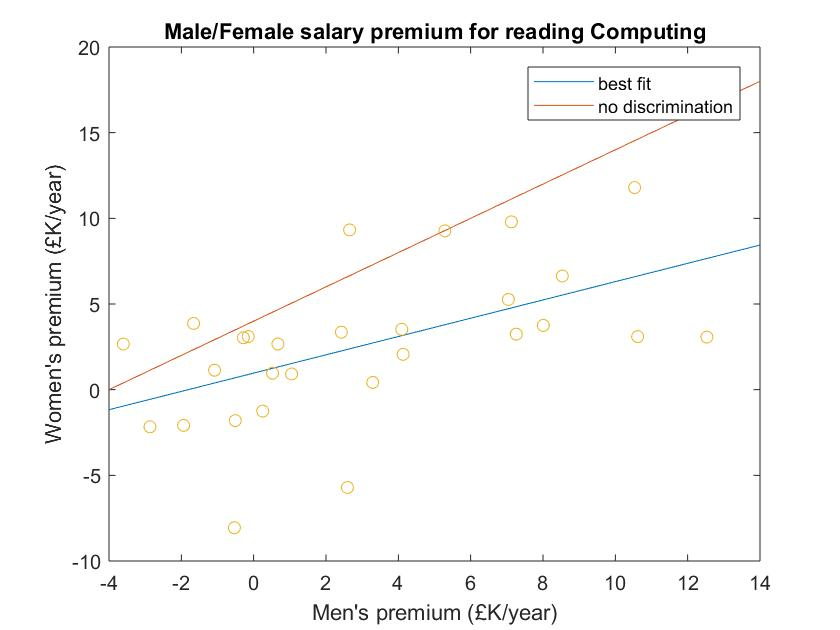
\includegraphics[scale=0.34]{BBCSalaryDatav4.jpg}}
\end{figure}
%Overall framing for the paper, etc

